\documentclass{report}
\usepackage[utf8]{inputenc}
\usepackage{hyperref}
\usepackage{setspace}
\usepackage{float}
\title{Universal Parabolic Constant}

\author{Balakrishnan Rajagopal (40075977) }
\date{}
\renewcommand{\baselinestretch}{1.15}

\usepackage{natbib}
\usepackage{graphicx}

\usepackage[final]{pdfpages}


\usepackage{fancyhdr}
\usepackage[margin=1in]{geometry}
\usepackage{pdfpages}
\renewcommand{\headrulewidth}{0.1pt}
\fancyhf{} 
\renewcommand{\headrulewidth}{0.1pt} 
\fancyfoot[C]{\thepage} 
\renewcommand{\footrulewidth}{0.1pt} 


\begin{document}
\maketitle


\newpage\chapter{Activity Diagram}
\section{Description}
The user enters the operands and the operator. Here, we have considered universal parabolic constant as the second operand. Once the user clicks equal operator, corresponding operations will be performed on operands.

\begin{itemize}
    \item If the user selects the "Add" function then the first and constant value will be added
    \item If the user selects the "Subtract" function then the constant will be subtracted from the first number.
    \item If the user selects the "Multiply" function then the first and constant value will be Multiplied
    \item If the user selects the "Divide" function then the first will be divided by the constant.
\end{itemize}
Finally, results will be displayed.

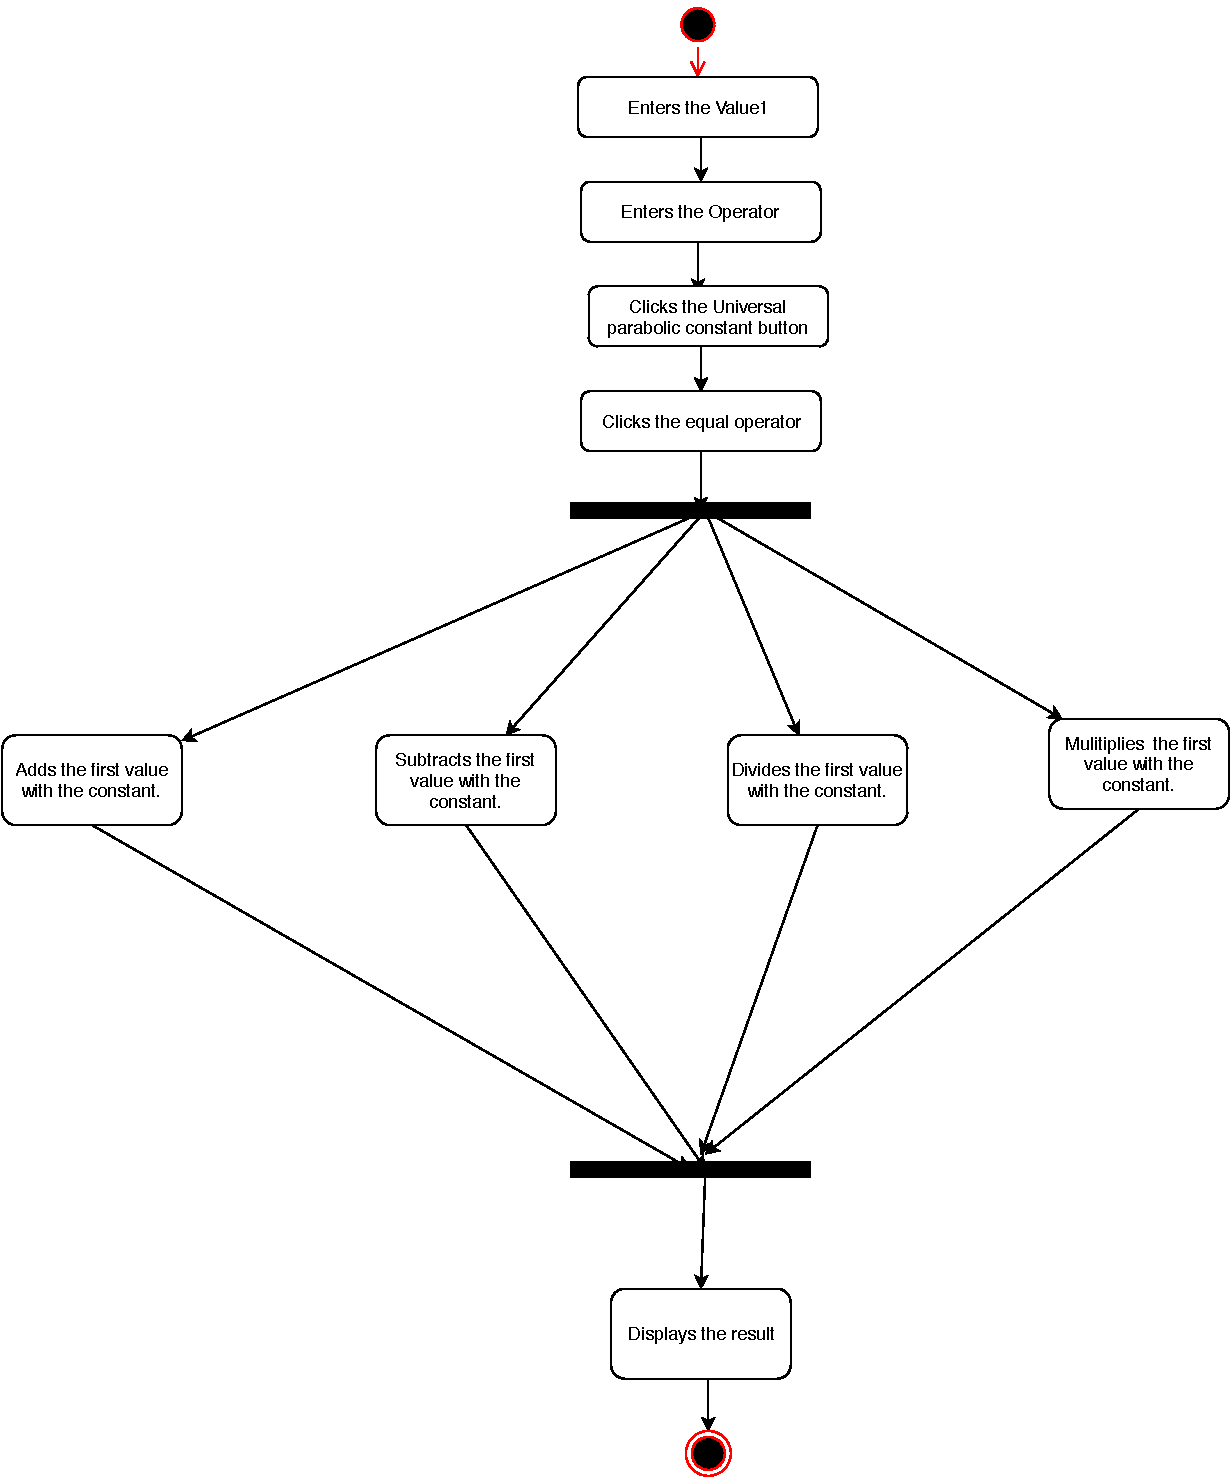
\includepdf[pages=1]{Activity.pdf}
\newpage
\newpage
\chapter{Use Case Diagram}

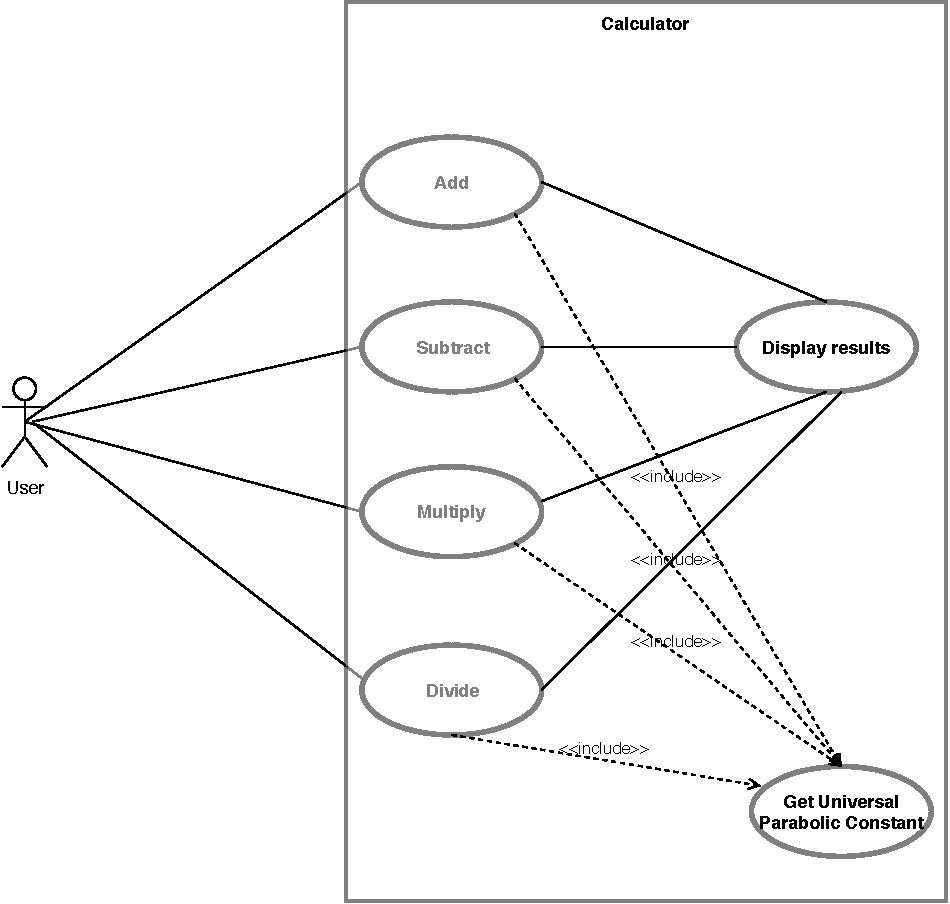
\includepdf[pages=1]{usecase.pdf}
\section{Description}
\begin{itemize}
    \item The goal of the "Add" Use case is to add the two numbers. 
    \item The goal of the "Sub" Use case is to subtract the two numbers. 
    \item The goal of the "Multiply" Use case is to Multiply the two numbers. 
    \item The goal of the "Divide" Use case is to divide the two numbers.
    \item The goal of the "Get Universal Parabolic Constant" Use case is to get the constant.
\end{itemize}
Finally, the goal of the "Display" use case is to display the results of the calculation.

\bibliographystyle{plain}
\bibliography{references}
\end{document}